\newcommand{\FigTheoryMuonDecayCloudChamber}{
\begin{figure}[tb]
\centering 
%\fbox{
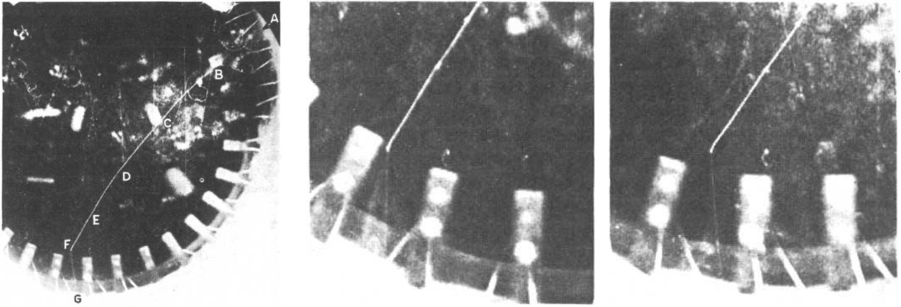
\includegraphics[width=0.95\textwidth]{figs/theory/EarlyCloudChamberMuonDecay.pdf}
%}
\caption[One of the earliest cloud chamber photographs of a muon, taken in 1940~\cite{Williams1940102}.]{
One of the earliest cloud chamber photographs of a muon, taken in 1940~\cite{Williams1940102}.
In the left-most image the muon enters the chamber at point A and travels to point F, where it eventually decays to an electron which can be seen faintly leaving the image at point G.
The images to the right are a stereoscopic zoom in on point F, showing the relatively slow and more ionising muon and the faster, less ionising electron.
\figlabel{theory:muonCloudChamber}}
%\footnote{though the author has failed to reproduce the stereoscopic effect with his own eyes}
\end{figure}
}

\newcommand{\FigTheoryHincksPontecorvoMuEGamma}{
\begin{figure}[tb]
\centering 
%\fbox{
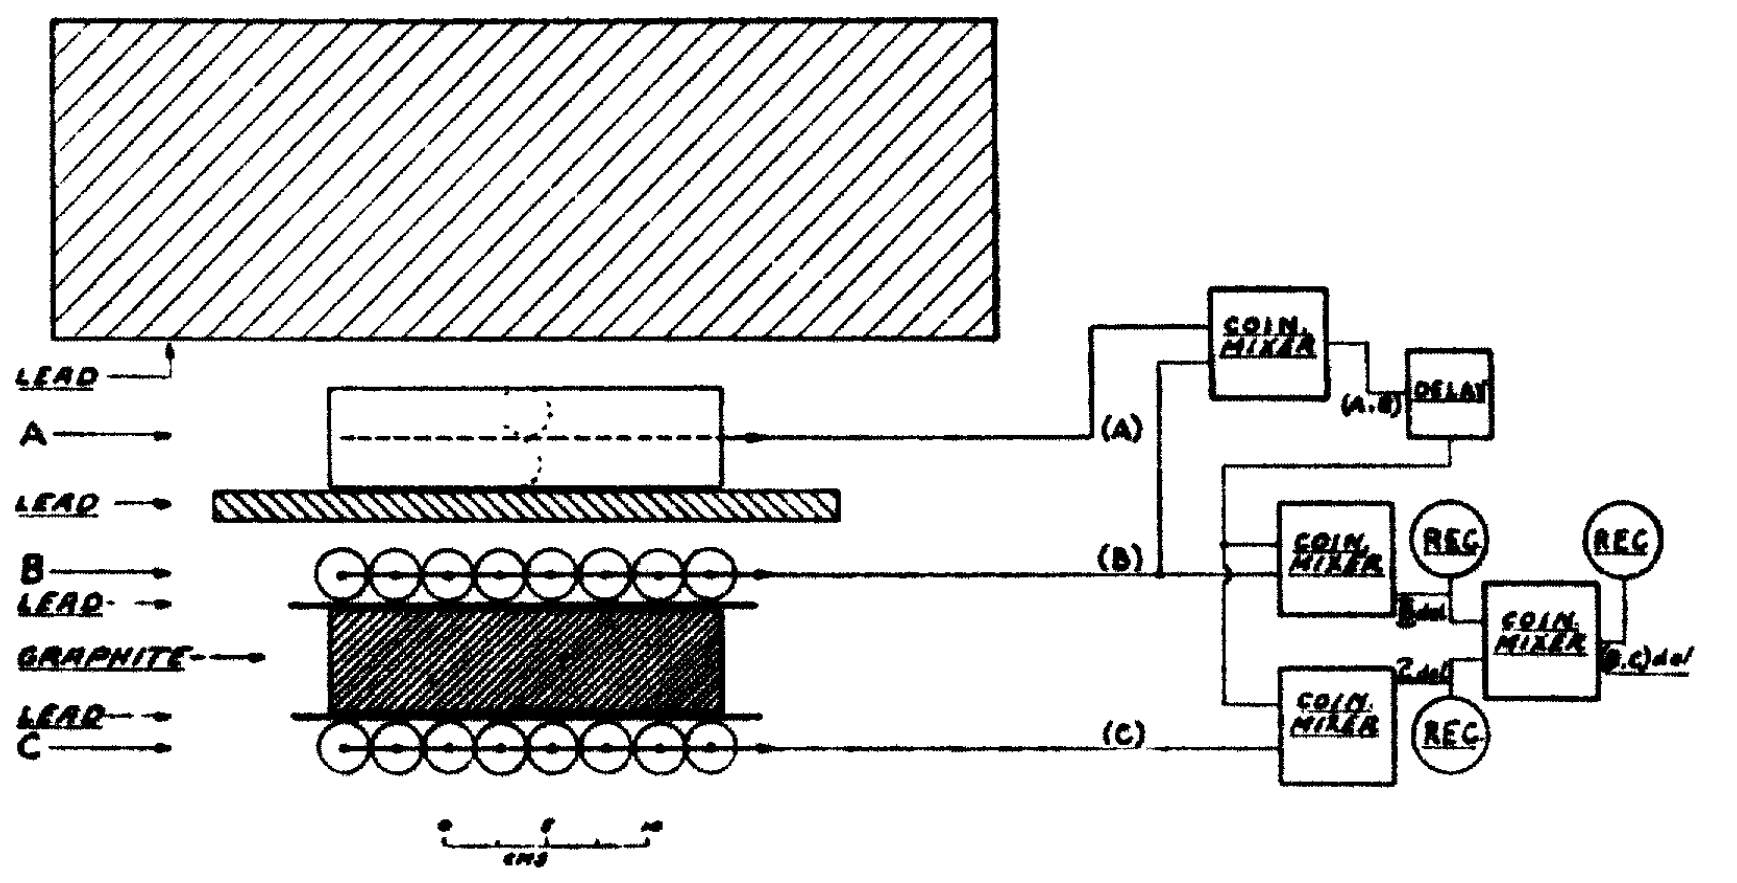
\includegraphics[width=0.85\textwidth]{figs/theory/OriginalMuEGammaExperiment.png}
%}
\caption[The setup of the first experiment to look for photons produced during muon decay taken from~\cite{Hincks194802}.]{
The setup of the first experiment to look for photons produced during muon decay taken from~\cite{Hincks194802}.
Cosmic muons arrived from the top, slowing down in the big block of lead, triggering two Geiger-Muller counters (A and B) as they passed and eventually coming to stop in the graphite.
From there, electrons and any potential photons would be detected in the counters above and below the graphite (B and C).  
No photons were seen in coincidence with an electron from muon decay, which lead theorists to hypothesise two distinct neutrino flavours.
\figlabel{theory:originalMEG}}
%\footnote{though the author has failed to reproduce the stereoscopic effect with his own eyes}
\end{figure}
}

\newcommand{\FigTheoryMuEGammViaNeutrino}{
\begin{figure}[t]
\centering 
%\fbox{
%\input{figs/feynman/mu_to_e_gamma_via_SM-Wgamma.tex}
\subfloat[][\figlabel{theory:feyn:muDecay}\ac{SM} Muon Decay]{\includegraphics[width=0.45\textwidth]{figs/feynman/pdfs/mu_decay.pdf}}\hspace{0.03\textwidth}
\subfloat[][\figlabel{theory:feyn:muEGammaViaNu}Neutrinoless Muon Decay with Photon Emission]{\includegraphics[width=0.45\textwidth]{figs/feynman/pdfs/mu_to_e_gamma_via_SM-Wgamma.pdf}}
%}
\caption[Feynman diagrams for Standard Model muon decay and neutrino oscillation-mediated \mutoe gamma]{
%Feynman diagram for the neutrinoless muon decay to a photon and electron mediated by a neutrino oscillation
The outgoing neutrinos produced in the \ac{SM} decay \protect\subref{fig:theory:feyn:muDecay} can be made into an internal neutrino propagator \protect\subref{fig:theory:feyn:muEGammaViaNu} via neutrino oscillations, whilst the addition of a photon ensures conservation the 4-momentum.
Although allowed in the \ac{SM} with neutrino oscillations, the actual rate from such a diagram is well below present experiment sensitivities.
A similar diagram was envisaged to show that the lack of observation of \mueg implied distinict neutrino flavours.
\figlabel{theory:feyn:decay}}
%\footnote{though the author has failed to reproduce the stereoscopic effect with his own eyes}
\end{figure}
}

\newcommand{\FigTheoryMuLFVLimits}{
\begin{figure}[tb]
\centering 
%\fbox{
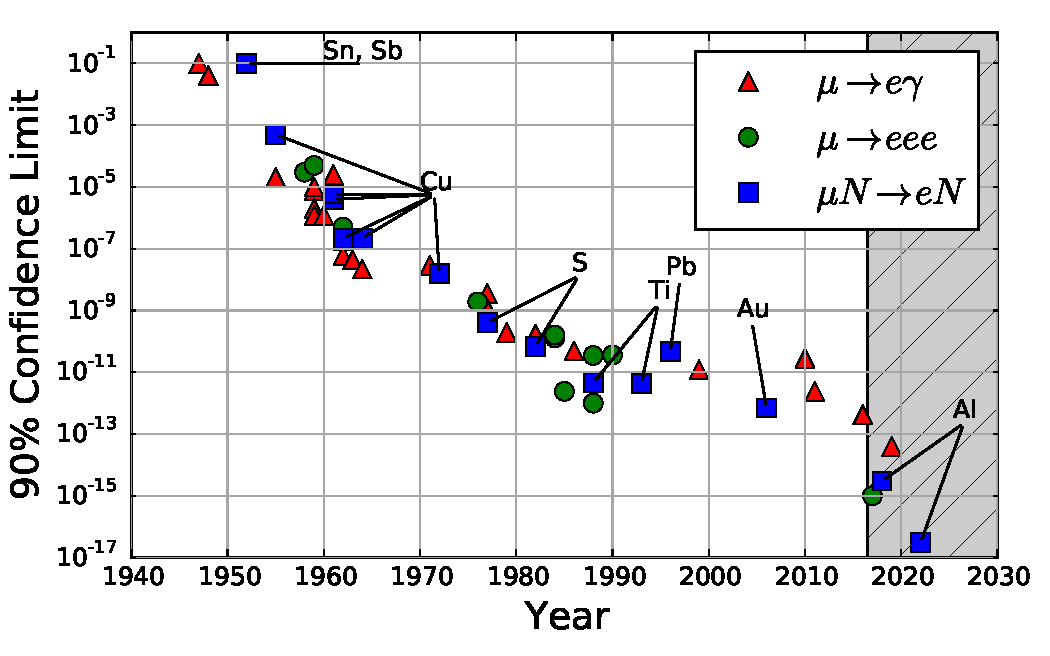
\includegraphics[width=0.95\textwidth]{figs/theory/MuLFVSearchLimits.pdf}
%}
\caption
[The historic evolution of experimental upper limits on \ac{CLFV} in muon channels]{
The experimental limits on \ac{CLFV} in muon channels has been reduced by some 13 orders of magnitude since the first search in 1947.
Each improvement in the limit is primarily due to the increasing intensity of the muon source:
cosmic muons were used around 1950; accelerator-produced muons followed; surface muon sources further increased the intensity; and nowadays superconducting solenoids will capture and focus the resulting muon beam.
%The improvements in the limit are primarily linked to the intensity of the available muon source: around 1950 cosmic muons were used; accelerator-based muon sources improved this, 
The shaded grey region shows measurements that are currently under preparation.
%, including MEG-II, Mu3e, Mu2e, and COMET \phaseI and \phaseII.
Data until 2015 is taken from the summary tables from~\cite{Bernstein2013hba}.
\figlabel{theory:muModesLimits}}
\end{figure}
}

\newcommand{\FigTheoryMuEConvViaNeutrino}{
\begin{figure}[t]
\centering 
%\fbox{
%\input{figs/feynman/mu_to_e_gamma_via_SM-Wgamma.tex}
\subfloat[][\figlabel{theory:feyn:muecViaNu:W}$\gamma$ Penguin]  {\includegraphics[width=0.43\textwidth]{figs/feynman/pdfs/mu_e_conversion_via_SM-Wgamma.pdf}}\hspace{0.08\textwidth}
\subfloat[][\figlabel{theory:feyn:muecViaNu:Z}$Z$ Penguin]  {\includegraphics[width=0.43\textwidth]{figs/feynman/pdfs/mu_e_conversion_via_SM-nuZ.pdf}}\\
\subfloat[][\figlabel{theory:feyn:muecViaNu:d}$d$-quark Box]{\includegraphics[width=0.43\textwidth]{figs/feynman/pdfs/mu_e_conversion_via_SM-downBox.pdf}}\hspace{0.08\textwidth}
\subfloat[][\figlabel{theory:feyn:muecViaNu:u}$u$-quark Box]{\includegraphics[width=0.43\textwidth]{figs/feynman/pdfs/mu_e_conversion_via_SM-upBox.pdf}}\\
%}
\caption
[Feynman diagram for the neutrinoless muon decay in the presence of an atomic nucleus---\mueconv{}---caused by neutrino oscillations.]{
Feynman diagram for the neutrinoless muon decay in the presence of an atomic nucleus---\mueconv{}---caused by neutrino oscillations.
Compared to \mueg there are now four possible diagrams, so that the rate depends on the nucleus and picks up interference terms.
\figlabel{theory:feyn:muecViaNu}}
%\footnote{though the author has failed to reproduce the stereoscopic effect with his own eyes}
\end{figure}
}


\newcommand{\FigTheoryMuEConvNewPhysics}{
\begin{figure}[tb]
%\vskip1cm
\centering
\subfloat[][\figlabel{theory:feyn:muecNP:HiggsDirect}Exotic Higgs]{ \includegraphics[width=0.16\textheight]{figs/feynman/pdfs/mu_e_conversion_Higgs.pdf}}\hspace{0.045\textwidth}
\subfloat[][\figlabel{theory:feyn:muecNP:Zprime}$Z$-prime]{         \includegraphics[width=0.16\textheight]{figs/feynman/pdfs/mu_e_conversion_Z_prime.pdf}}\hspace{0.045\textwidth}
\subfloat[][\figlabel{theory:feyn:muecNP:Leptoquark}Leptoquarks]{   \includegraphics[width=0.16\textheight]{figs/feynman/pdfs/mu_e_conversion_Leptoquark.pdf}}\\
\subfloat[][\figlabel{theory:feyn:muecNP:HeavyN}Heavy Neutrinos]{   \includegraphics[width=0.2\textheight]{figs/feynman/pdfs/mu_e_conversion_via_heavy_neutrino.pdf}}\hspace{0.02\textwidth}
\subfloat[][\figlabel{theory:feyn:muecNP:HiggsTopLoop}Exotic Higgs]{\includegraphics[width=0.17\textheight]{figs/feynman/pdfs/mu_e_conversion_HiggsTopLoop.pdf}}\hspace{0.02\textwidth}
\subfloat[][\figlabel{theory:feyn:muecNP:SUSY}Supersymmetry]{       \includegraphics[width=0.2\textheight]{figs/feynman/pdfs/mu_e_conversion_via_susy.pdf}}\\
%\subfloat[][\label{fig:FD-Z-h}Z-prime and extended Higgs]{\input{feynman/mu_e_conversion_Z_prime}}
\caption
[Feynman diagrams that produce \mueconv through New Physics models.]{
Feynman diagrams that produce \mueconv through New Physics models.
The upper three diagrams (\protect\subref{fig:theory:feyn:muecNP:HiggsDirect} to \protect\subref{fig:theory:feyn:muecNP:Leptoquark}) all connect to the nucleus via some massive exchange particle, 
whereas the lower three diagrams (\protect\subref{fig:theory:feyn:muecNP:HeavyN} to \protect\subref{fig:theory:feyn:muecNP:SUSY}) all connect via an exchanged photon.
In addition to interactions with the quarks, since \mueconv interacts with the whole nucleus, there are also models where the interaction involves external gluon lines.
\figlabel{theory:feyn:muecNP}}
\end{figure}
}

\newcommand{\FigTheoryMuecVsMueg}{
\begin{figure}[tb]
\centering 
%\fbox{
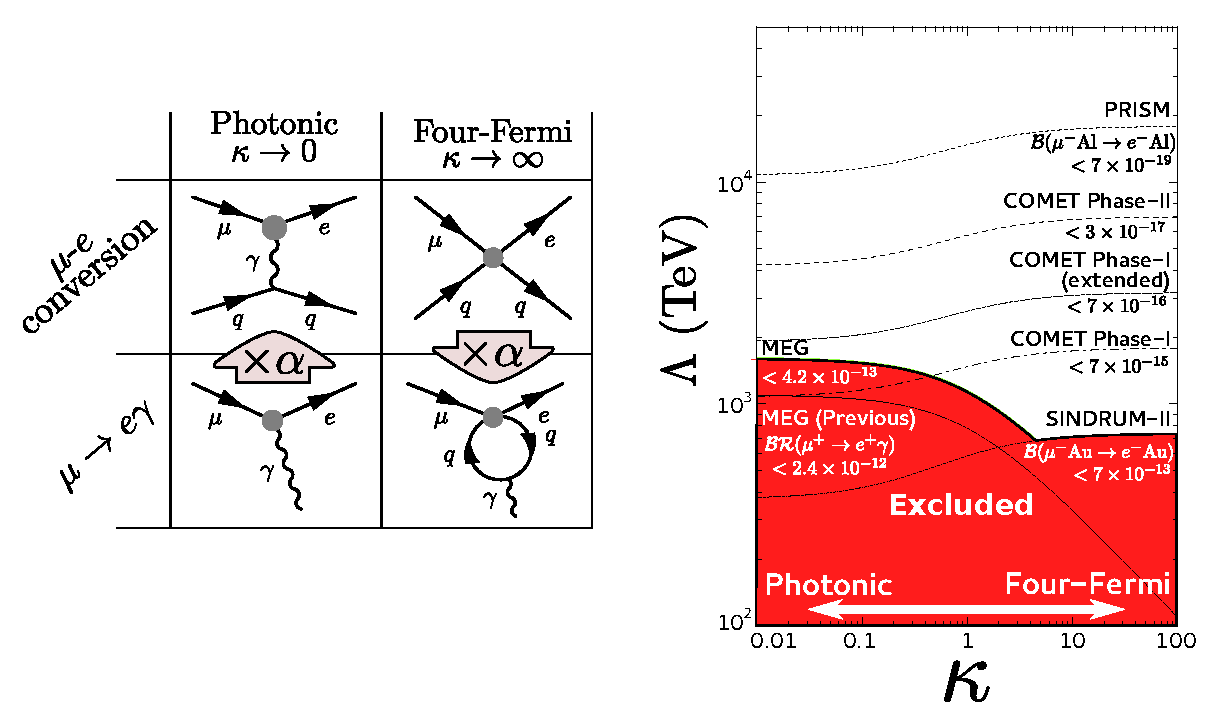
\includegraphics[width=0.95\textwidth]{figs/theory/MuecVsMueg.pdf}
%}
\caption
[Comparison of \mueconv and \muegamma]{
Searches for \mueconv and \muegamma have relative sensitivities that depend on the underlying physics, making the two channels highly complementary.
As shown on the left, New Physics can produce a signal in both channels, but one channel or the other can be comparatively suppressed due to the need to include extra vertices and loops.
The plot on the right is adapted from~\cite{ProposalPhase1}, based on~\cite{DEGOUVEA2009303}, and shows the relative sensitivity for the toy lagrangian of equation~\eq{theory:toy} as a function of $\kappa$, how non-photonic the New Physics is, and $\Lambda$, the mass scale assuming coupling strengths of unity.
\figlabel{theory:muecVsMueg}}
%\footnote{though the author has failed to reproduce the stereoscopic effect with his own eyes}
\end{figure}
}


\chapter{The History and Theory of \acf{CLFV}}
\chapterquote{Who ordered that?}{The author upon presentation of `ika-no-ikizukuri' (live squid sashimi) at a collaboration meeting in Fukuoka, Kyushu Island}
%\begin{easylist}
%# "Who ordered that?" -- The author upon presentation of `ika-no-ikizukuri' (live squid sashimi), in Fukuoka, North Kyushu
%	## Not predicted before observation
%	## Neutrino masses and oscillations one of the only observations of our time not to have been predicted
%	## 
%# History of the muon and its importance to the development of the standard model
%	## Early searches for mu to e gamma,
%	##	multiple neutrino flavours,
%	##	observation of muon neutrino
%# Lepton Flavour: Neutrinos and the Charged Leptons
%# Neutrino oscillations, PMNS matrix, neutrino masses,
%# Charged Lepton Flavour Violation searches
%	## Theoretical motivation
%	   ### Lepton non-universality => CLFV
%	   ### Baryon asymmetry
%	   ### Neutrino mass generation and scale
%	## Example models: SUSY
%	## Example models: neutrino seesaw? 
%	## Observables and current limits
%	## Interplay between mu-e conversion and mu -> e gamma experiments
%# Muon-to-electron Conversion and the Physics of Muonic Atoms
%\end{easylist}
\section{The Muon and the Birth of the Standard Model}
%At the turn of the 20\textsuperscript{th} century, physics felt itself on confident ground.
%Newton's laws of mechanics had been applied to large ensembles of particles producing the statistical theory of thermodynamics which had driven the industrial revolution.
%Maxwell had unified the electric and magnetic fields which led to the development of electricity and electrical components such as capacitors and inductors.
%For a while the theory of electromagnetism was in tension with Newton's mechanics and the concept of an invisible omnipresent `aether' seemed a reasonable explanation.
%The Michelson-Morley experiments, however, laid this to rest proving light to travel at the same speed regardless of the speed of the observer or source.
%It was not long though before Einstein, working in his patent office, used this to develop the theory of special relativity.
%
%Around the same time, the ultra-violet catastrophe that predicted infinite energy be emitted due to the heat of an object in the ultra-violet part of the spectrum was solved by Planck, bringing the quantisation of light and the concept of a photon.
%It was Einstein again who used this to explain the photo-electric effect that eventually won him the Nobel prize.
%Finally, it was the explanation of the hydrogen atom's emission spectrum by Bohr, using de Broglie's concept of an electron wave, and the theory of quantum mechanics was born.
%
%At this point, atoms were made of neutron, protons and electrons, coming a long way from the plum-pudding 
%
%----
%
%In the early 1930's, physicists felt themselves on confident ground, having completely rewritten the physics textbook during the last quarter century.
%On large scales, 400 year old Galilean invariance had given way to special relativity, whilst Newtonian mechanics and gravity had fallen to the general theory of relativity.
%And on the tiniest of scales, quantum mechanics had revolutionised the behaviour (and our philosophy) of matter and energy.
%Electrons, protons, and neutrons were the children that filled the playing field of this new school, as well as the photon which often made appearances.
%
%Electrons were known to hang around protons and neutrons which themselves were normally found in even more tightly-bound `nuclei'.
%The electromagnetic attraction that the electrons felt for the protons (and therefore the nucleus as a whole, given the neutrons' electromagnetic indifference) was well understood.
%Theories existed to explain why occasionally a neutron would be seen to change into a proton, releasing an electron in the process.
%Other theories were also able to explain the strong force that seemed to keep the protons and neutrons together, proposing a new member that would appear and disappear quickly enough that no-one outside the nucleus would see it.
%
%This theory had been proposed by one Yukawa~\cite{Yukawa}
%
%----
%
%I remember being a school student and asking my chemistry teacher was how the nucleus of an atom, consisting only of positive protons and neutral neutrons, was able to stay together despite the repulse electrostatic forces.
%It was a slightly loaded question, since I already knew of the strong force, but I hoped that at he would enlighten me as to how it worked.
%I did not know this then, but physicists in the 1930s had asked almost the identical question, realising there must be some additional force that holds the protons together.
%
%One Japanese physicist, Hideki Yukawa,suggested this force was mediated by some particle being exchanged between the protons and neutrons, in a similar way to how the electromagnetic force was known to exist via photon exchanges.
%If this new particle were to be massive and unstable then one could explain how such a strong force would die off so quickly away from the nucleus.
%Better yet, Yukawa was able to estimate the mass of this exchange particle via the uncertainty principle and even predicted how long it should live for: it should be about 100~MeV and live for around $10^{-8}$ seconds \CHECK{Are these the correct values?}.
%
%Then in 1937, a particle with very close to this mass was discovered from cosmic ray events.
%Surprisingly though, the discovered particle lived for around $10^{-6}$ seconds -- much longer than predicted by Yukawa's model, prompting Rabi to make the famous quote that 
%------

%\begin{easylist}
%    # Turn of the century, phsyics nearly complete
%    ## Complete picture of protons, neutrons, electrons
%    ## Suggestion of short-lived meson to mediate the strong force that bound the nucleus together
%    ## Weak force that would sometimes change protons and neutrons but conserve isospin
%    # First un-predicted particle of the SM: Muon
%    ## Long-lived meson but with a mass close to requirement for strong force mediator
%    ## Only decayed to an electron
%    ## Electron had a spectrum of energies, similar to beta-decay measurements
%    ## Massless neutrinos used to explain beta-decay to conserve 4-momentum
%    ## Now need two distinct neutrino flavours and the conservation of flavour conservation
%    ## Searches for the second type of neutrino flavour proved fruitful
%    ## Searches for muon decay to an electron with a photon were unsuccesful
%    # Lepton flavour conservation
%    ## Noethers Theorem: Continuous symmetry generates a conseved current: eg. Electric charge, momentum, energy, total angular momentum
%    ## No such symmetry for lepton flavour
%    ## Embedded in the electroweak theory
%    ## Yukawa couplings and the CKM matrix (I feel uncertain about this, but since I should know it anyway, it's perhaps something I include briefly then make sure to revise before the viva).
%\end{easylist}
In 1897, the British physicist Thomson discovered the first sub-atomic particle: the electron.
In the next 30 years or so, the supposedly indivisible object of the atom was divided multiple times, giving way to the neutron, the proton, and the first of their anti-particles soon to be known as the positron.
Far from the simple, solid sphere previously assumed, the atom had become a dynamic object, with a cloud of negative electrons bound to a positive nucleus consisting of neutrons and protons.

That the electrons were bound to the nucleus was readily understood due to their opposite electric charges.
What it was that occasionally turned a proton into a neutron, or vice versa, and in the process emitting an electron was less clear.
And the nucleus itself posed still another challenge, in that something had to be overcoming the repulsion between the like-charged protons.

In 1935, Yukawa -- a physicist from Japan, where this thesis will often return -- proposed that, as for the electromagnetic force binding electrons to the nucleus via the exchange of some carrier particle (the photon), 
an exchanged particle could explain the very strong force that helped to glue protons to neutrons forming the nucleus.
Unlike the photon though, this particle would be have to be massive and readily absorbed to the protons and neutrons.
Yukawa was even able to predict the mass of this particle via the uncertainty principle, finding it to be around 100~MeV~\cite{}.

\FigTheoryMuonDecayCloudChamber
Then, in 1937, a particle with a mass very close to this prediction was observed in cosmic ray events by several physicists in Japan~\cite{Nishina193712} and the US~\cite{Neddermeyer1937md,Street193711}.
But the initial hopes that this was indeed the Yukawa particle faded quickly as this particle easily penetrated through the matter of the detectors, whilst Yukawa's particle should be rapidly absorbed.
So unexpected was this new particle with its mass in between that of an electron and a proton and its relatively long lifetime, that Rabi was also forced to ask, ``Who ordered that?'
It took some time, but eventually this particle became known as the muon.

The muon was interesting because it seemed to interact very weakly with matter, and because it seemed only to decay to an electron.
%Given that an electron has 0.511~MeV, about 200 times lighter than a muon, the obvious question was how the muon was decaying to an electron.
For this to happen, something else has to be emitted in order to conserve momentum and energy, given that the electron is about 207 times lighter than the muon.
There were two obvious possibilities for the `something else': a photon, or a neutrino-antineutrino pair.

Neutrinos were particles that had up to now been a theoretical tool to help explain beta decay.
Beta decay occurs when a nucleus emits an electron or positron and in so doing swaps a neutron for a proton or a proton for a neutron.
The difference in the mass between the original and final nucleus was a fixed value, and yet electrons were seen with a range of energies all less than the value of this difference.
The neutrino was proposed as a solution: a massless particle was carrying away the missing energy and had the additional property of interacting only very weakly making it nearly impossible to detect.
By studying the spin of the parent and daughter nucleus it was also that the neutrino had spin of $\hbar/2$.

%For the decay of the muon there were both similarities and differences with beta-decay.
%Similarities because it only produced electrons with a range of energy less than the mass of the muon.
%Differences because the range of energies could not really be explained by the production of a single neutrino.
%By conservation of total angular momentum, the number of neutrinos had to be two.

Muon decay was similar in that the electron appeared with less energy than was available to it, but different because it appeared from the spectrum of electrons that not one but two neutrinos were being emitted.
Being spin half particles, either the neutrino was its own anti-particle, or one would be a neutrino and the other an anti-neutrino.
Either way, having two neutrinos emitted posed its own challenge since the two neutrinos would be able to annihilate with one another, and muon decay to a photon and electron would become comparably large.
Searches for a muon decaying to a photon and electron were performed~\cite{Hincks194802}, but came back empty handed;
clearly something else, something new, had to be introduced to distinguish one neutrino from the other, such that they were unable to annihilate one another.
\FigTheoryHincksPontecorvoMuEGamma

This something became known as 	`lepton flavour'.  
One neutrino carried away the `flavour' of the muon, the other carried the `flavour' of the electron.
If you start out with a muon, you must keep either a muon or a muon-neutrino; if you start with an electron you must finish with an electron, or an electron-neutrino.
This is nowadays known as lepton flavour conservation and was cemented into theory when muon-neutrinos were identified in an experiment at Brookhaven that saw muons being produced from the neutrinos originally emitted when
a pion (the modern name for Yukawa's particle) decays to a muon~\cite{MuNeutrinoDiscovery}.
Thus the discovery of the muon had not only provided a new charged particle, but also a new type of neutrino and a new law of conservation!

Noethers theorem tells us that for every system with a continuous symmetry, some quantity will remain conserved.
This is the rule that gives us conservation of momentum, energy and angular momentum (the conserved properties) in systems that are the same regardless of their place, time, or direction (the continuous symmetries).
An extension of this theorem applies for local transformations of the system's `gauge', which is any property that when changed has no impact on the physics outcome, such as the absolute value of the ground in an electric circuit.
In particle physics, this extension gives rise to the various particle charges, such as the electromagnetic charge caused by the $U(1)$, or simple phase, of a particle's wavefunction and the even more abstract $SU(2)$ and $SU(3)$ hypercharges of the weak and strong (colour) forces.
In the case of the conservation of lepton flavour however, no such symmetry exists.
Instead, this conservation is embedded into the \ac{SM} of particle physics through the electroweak theory and lepton universality.

In addition to the leptons and their interactions via the electroweak forces, the \ac{SM} describes the quark sector and their interactions via \ac{QCD}.
Quarks are the particles that make up the neutrons and protons (not only have we divided the atom, but also its constituents) and even the pion, Yukawa's predicted particle that was discovered in 1947.
Built around the frameworks of local gauge invariance, quantum field theory, and spontaneous symmetry breaking, the \ac{SM} has been one of the most rigorously tested theories, and with only a few exceptions has held up incredibly well to measurements so far.

\section{Neutrino Oscillations Break Lepton Flavour Conservation}
%\begin{easylist}
%    # Break lepton flavour conservation
%    # Neutrinos have mass
%    # PMNS matrix, similar to CKM matrix but with very different form
%    # Additional source of CP violation, good for baryon asymmetry?
%    # Majorana neutrinos?
%    # Charged lepton flavour violation via neutrinos
%    ## Mu to e gamma via a neutrino-W loop
%    ## \mueconv via neutrino loops
%\end{easylist}
In the 1970s, evidence began to emerge that the concept of Lepton Flavour Conservation might have holes.
Raymond Davis Jr.\ and his group at Brookhaven measured the number of electron neutrinos coming from the sun and found there to be about one third too few~\cite{}.
This puzzle remained until it was solved by experiments in Canada and Japan in the early 2000s: the neutrinos were being produced in the expected quantity but as they travelled from where they were produced to the detectors on earth, they were changing their flavour!
Nowadays, experiments in Japan and the US, such as the T2K experiment~\cite{T2K:nim} and Nova~\cite{}, produce beams of muon neutrinos only to detect them hundreds of kilometres away as electron neutrinos.

Explaining this requires that neutrinos have mass, although far less than any other of the particles in the \ac{SM}.
Not only that, but the neutrino states with definite mass are not the same as the flavour states by which neutrinos interact with everything else.
Since it is the mass eigenstate that determines a particle's propagation but the flavour eigenstate that determines the neutrino's interaction, an oscillation occurs where the probability of detecting a neutrino in a given flavour state depends on how far it has propagated since production.
\FigTheoryMuEGammViaNeutrino

As for the discovery of the muon, the unexpected discovery \CHECK{was it?} of non-zero mass of the neutrino and the mixing between flavour states has opened a whole host of new questions.
How does the neutrino acquire its mass?
  Why is the mass scale so much smaller than any other known particle?
As the only chargeless, massive fermion in the \ac{SM}, what is the nature of this mass:
Is it produced via an interaction with the Higgs or via a Majorana mechanism, in turn making the neutrino into its own antiparticle?
Is it a combination of these mechanisms?

\FigTheoryMuEConvViaNeutrino
Either way it is clear that the neutrinos themselves do not conserve lepton flavour, and this immediately makes it possible that the charged leptons -- the electron, the muon, and the tau -- also break Lepton Flavour Conservation.
How neutrinos cause this is demonstrated in \fig{theory:feyn:muEGammaViaNu}, where the muon neutrino annihilates with the electron neutrino whilst energy and momentum are conserved by the emitted photon.
The fact this was not seen motivated lepton flavour in the first place, and yet now we know it to be possible.
However, we can now calculate the rate for such a diagram and find it to be heavily suppressed:
\begin{equation}
\mathcal{BR}(\mu\rightarrow{}e\gamma)\propto\left|\sum_iU^*_{\mu i}U_{ei} \frac{m^2_{\nu_i}}{M^2_W}\right|^2 < 10^{-54},
\end{equation}
where $U_{\alpha i}$ is an element of the mass-mixing matrix transforming the $\alpha$ flavour state to the $i$-th mass state with mass $M_{\nu_i}$, and $M_W$ is the mass of the $W$-boson.
This rate can be considered double suppressed: the summation over the different mass eigenstates produces a GIM suppression, whilst the mass imbalance between the neutrinos and the $W$-boson suppresses this further.

Emission of a photon is not the only process made possible by neutrino oscillations and \ac{LFV}.
A negative muon that has become bound to the nucleus of an atom (discussed further in \sect{theory:atomicMuon}) will also be able to convert to an electron without emitting neutrinos via the diagrams
shown in \fig{theory:feyn:muecViaNu}.  
In this case however, the rate calculation is complicated by the quark contents of the nucleus, form factors of the quarks in the nucleons and nucleons in the nucleus, and the cancellations that occur between each diagram.

\section{In Search of \acf{CLFV}}
\subsection{Motivations and Status}
%\begin{easylist}
%    # Experimental searches
%    ## List of observables and current limits
%    ## Development of limits for muon LFV searches with time
%    ## Present experimental searches and hints
%    ## Attractiveness of searches with intense muon beams
%    # Importance of CLFV from a theoretical perspective
%    ## Baryon asymmetry
%    ## Minimal flavour violation
%    ## Neutrino mass generation
%    ## Lepton universality
%    # Models that generate \mueconv
%    # Complementarity between searches: \mueconv vs. \muegamma
%\end{easylist}
Searches for \ac{LFV} go back right to the discovery of the muon, but that is not to say that they ended there.
Over the past eighty years or so, experiments have continued to push the limits on such processes down through around 13 orders of magnitude.
As accelerator technology improved, rather than rely on cosmic sources, intense beams of muons can now be made and tau leptons generated at the large colliders.
\Tab{theory:currentLimits} shows the current limits on a (non-exhaustive) list of the possible \ac{CLFV} observables.

Of the searches involving muon decays the three most searched for modes have been \mueg (`mu to e gamma'), \muec (`\mueconv'), and \muThreeE (`mu three e').
From an experimental perspective these modes are attractive since the Lepton Flavour Conserving counterparts all have neutrinos in the final state, and since these neutrinos are massless they typically carry away around half the available energy.
By removing the neutrinos from the final state then a clear separation between the signal and the Standard Model version appears.
It is in these modes that the experimental limits have seen the greatest improvement with time, as shown in \fig{theory:muModesLimits}.

The \ac{SM} nowadays faces many other difficulties beyond neutrino masses such as dark matter and energy, the stability of the vacuum, and the unification of gravity, the electroweak force, and \ac{QCD}.
A vast number of extensions to the \ac{SM} try to address these issues.
The assumption that New Physics introduces no additional flavour changing is often referred to as Minimal Flavour Violation, and used to reduce the number of parameters contained in \ac{bsm} theories, but just how valid is such aan assumption?
As an accidental symmetry in the \ac{SM}, whether or not these extensions produce \ac{CLFV} is very difficult to constrain by some theoretical reasoning, and must instead be directly measured.

Beyond directly producing \ac{CLFV}, trying to answer the many questions raised by the small, non-zero neutrino masses is helped by searches for \ac{CLFV}.
In many of the proposed models, such as type-I see-saw mechanism \ac{CLFV} rates are significantly enhanced \CHECK{That's the right type of See saw mechanism, right?  Also add a citation}.
If heavy neutrinos exist they can remove both the GIM~suppression and the mass imbalance that cause the \ac{SM} with neutrino oscillation rates to be so small.

Lastly, there are a number of recent anomalies, in particular with muon measurements, that hint at \ac{CLFV}.
The experimentally measured value of $g-2$ of the muon has disagreed with the theoretical prediction by around 3~$\sigma$ for the last decade or two\CHECK{how long has this anomaly persisted for?}, even worsening as the theoretical prediction has been improved.
At the same time, measurements of the proton radius using the hyperfine structure of muonic hydrogen has shown a 4~$\sigma$ discrepancy~\cite{} with other methods.
Both of these could be explained by vacuum interactions of the muon with some new physics~\cite{}.

In addition, a number of collider-based measurements have turned up anomalies, such as the ratio of $B^+$ decays to a kaon and either a muon-antimuon pair or an electron-positron pair ($B^+\rightarrow K^+l^+l^-$), $R_K$, measured at both LHCb and the B factories~\cite{}.
This anomaly is echoed in LHCb's measurement of differential cross section of $B_s\rightarrow\phi\mu\mu$~\cite{} and the value of the $P'_5$ variable for $B\rightarrow K^*\mu\mu$.
Both ATLAS and CMS observed an excess in $h\rightarrow\mu e$ events during Run-1~\cite{} although this is yet to be confirmed during Run-2.
And although many of these discrepancies directly only require lepton non-universality, this can be shown to imply \ac{CLFV} in many cases~\cite{}.

Lastly, for cosmological purposes \ac{CLFV} can play an important role in the Baryon Asymmetry of the Universe that we observe.
Many models generate this asymmetry in the early universe via leptonic CP-violation.
However, it has been shown that if \ac{CLFV} processes occur at the present limits, the Baryon Asymmetry generated by these means can be washed out~\cite{}.
%\begin{easylist}
%# As an accidental symmetry in the SM, it cannot be constrained by some theoretical reasoning, purely by measurement
%# New physics then has nothing to prevent it predicting CLFV at any rate up to the experimental limit, thus searches for CLFV can confirm these theories or else rule them out and constrain them by setting more stringent limits.  Often theorists inject `Minimal Flavour Violation' but is this a valid assumption?
%# Giving the neutrino mass and simultaneously explaining why the mass should be so small compared to the other particles raises challenges and new predictions: very heavy neutrinos in a see-saw model.  These can remove the GIM suppression and the mass imbalance from the SM neutrino diagrams and therefore cause sizeable rates.
%# Lepton non-universality has been hinted at from several experimental sources: g-2 of the muon, Lamb shift of muonic hydrogen, the ratio of kaon and B decays with electrons or neutrinos.  Lepton non-universality in many models implies CLFV
%# Baryon asymmetry of the universe is hard to generate if CLFV exists
%\end{easylist} 

\subsection{Muon CLFV Channels}
\FigTheoryMuEConvNewPhysics
\Fig{theory:feyn:muecNP} shows a variety of Feynman diagrams for \mueconv involving new particles and couplings predicted by many \ac{bsm} theories.
The large variety of models to which \mueconv would be sensitive makes this a particularly attractive search channel for New Physics~\cite{Altmannshofer2009ne}.

It can also be seen how complementary the different muon CLFV channels will be.
In the case of leptoquarks for example, shown in \fig{theory:feyn:muecNP:Leptoquark}, clearly one would expect at some level \mueconv to take place, but to generate a signal in a \muThreeE experiment would be harder.
Similarly the relative sensitivities between \mueg searches and \mueconv searches can be used to pin down what the New Physics is in the case of a positive observation, or heavily constrain multiple different models in the case of a null measurement.
This is apparent from the fact that New Physics can be classed as photonic (such as the lower three diagrams in \fig{theory:feyn:muecNP}) or four-Fermi contact-like (like the upper three diagrams in \fig{theory:feyn:muecNP}).
In this case, the new physics which kicks in at some new mass scale is integrated away to leave an effective, low-energy field theory.

By constructing a toy Lagrangian consisting of two new interaction terms, one being photonic and the other a contact term it is possible to study the relative sensitivities of \mueconv and \mutoe gamma searches.
The interaction terms in such a Lagrangian would look like:
\begin{equation}
L=\frac{1}{\kappa+1}\frac{m_\mu}{\Lambda^2}\left(\bar{\mu}_R\sigma^{\mu\nu}e_LF_{\mu\nu}\right)+\frac{\kappa}{\kappa+1}\frac{1}{\Lambda^2}\left(\bar{\mu_L}\gamma^\mu e_L\right)\left(\bar{q_L}\gamma_\mu q_L\right)
\end{equation}

\section{The \mueconv process}
\sect{theory:atomicMuon}
\begin{easylist}
  # Coherent conversion, Signal, normalisation
  # Muonic atoms
  ## Formation and the electromagnetic cascade to the ground state
  ## Decay in orbit of bound muons
  ## Muon nuclear capture
\end{easylist}
